We demonstrate VIP in a variety of contexts including sensor
selection, Bayesian experiment design, and active learning.  The
comparison in each setting is to MCMC inference, or exact numerical
inference when possible, along with empirical mean estimation of the
MI for planning.  In this way, our motivation is to demonstrate
comparable accuracy using more efficient variational methods.  For the
more complex case of LLDA we in fact observe sustained improvements
over baseline.

\subsection{Sensor Selection}

We begin with estimating target position in a network of sensors, each
with fixed position.  Due to communication constraints we can draw
measurements from only a single sensor at each time.  At each planning
stage we must draw measurements from the most informative sensor.

%% We model sensor
%% noise as depending on the relative distance to the unknown target;
%% sensors further from the target produce less accurate detections.  

\textbf{Static Estimation.}  A stationary target has position drawn
from a Gaussian prior $x \sim \Ncal(m,\sigma^2)$.  Observations are
drawn from one of $K$ sensors, each with fixed position $l_k$.  Sensor
noise is modeled as a two-component Gaussian mixture model,
\[
  y \mid x; k \sim w * \Ncal(0, v_0) + (1-w) * \Ncal(x, v_k(x)).
\]
The mixture consists of a noise distribution with fixed variance $v_0$
and an observation model with noise variance increasing with relative
distance: \mbox{$v_k(x) = |l_k - x| + v_1$}.

\begin{figure}
  \begin{tabular}{cc}
    \hspace{-3mm}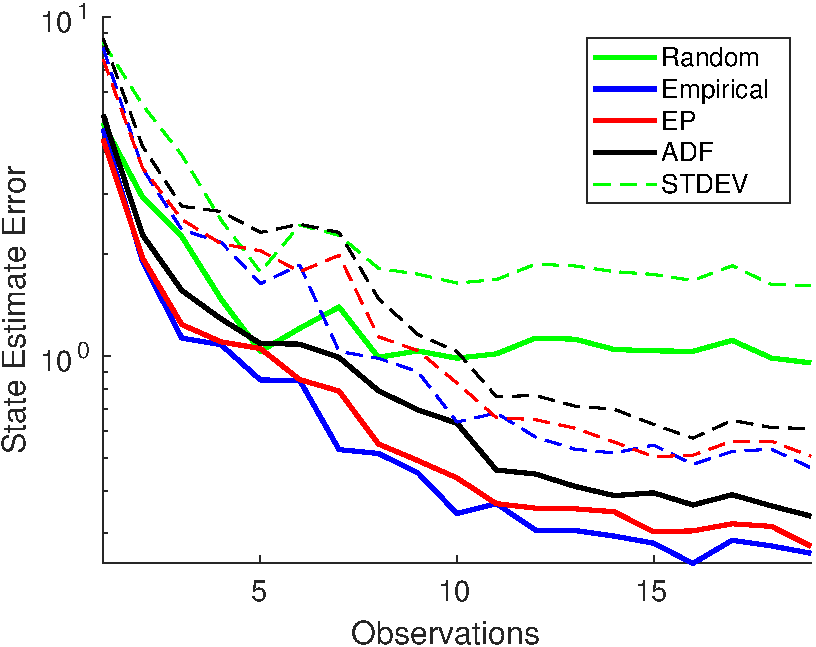
\includegraphics[width=0.24\textwidth]{ss_stateerr_maxIters100_Nsamp50_Nruns20.pdf} &
    \hspace{-5mm}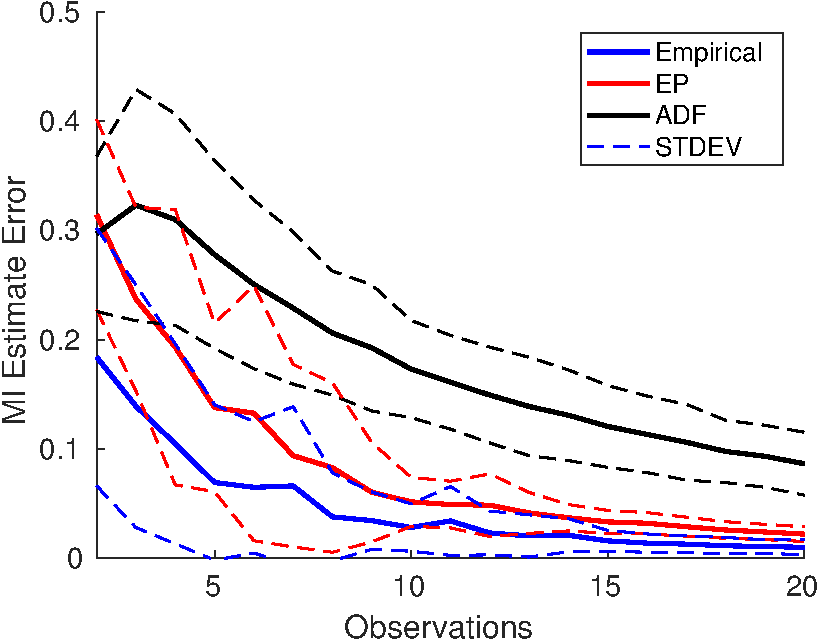
\includegraphics[width=0.24\textwidth]{ss_MI_maxIters100_Nsamp50_Nruns20.pdf}
  \end{tabular}
  
  \caption{\small\textbf{Static target estimation.} Estimation of a 1D
    target position in a network of $K=10$ equally spaced sensors.
    Mean (solid) plus STDEV (dashed) over 20 realizations.  \emph{Left:}
    Variational planning based on EP inference yields comparable error
    in state estimate compared to exact inference with empirical MI
    estimates. ADF inference yields higher error.  \emph{Right:}
    Empirical estimates based on the numerical posterior most
    accurately estimate MI.  VIP bound gap is consistently lower for
    more accurate EP posterior estimates as compared to
    ADF.}  \label{fig:static}
\end{figure}

\begin{figure*}[!t]
  \centering
  \hspace{-3mm}
  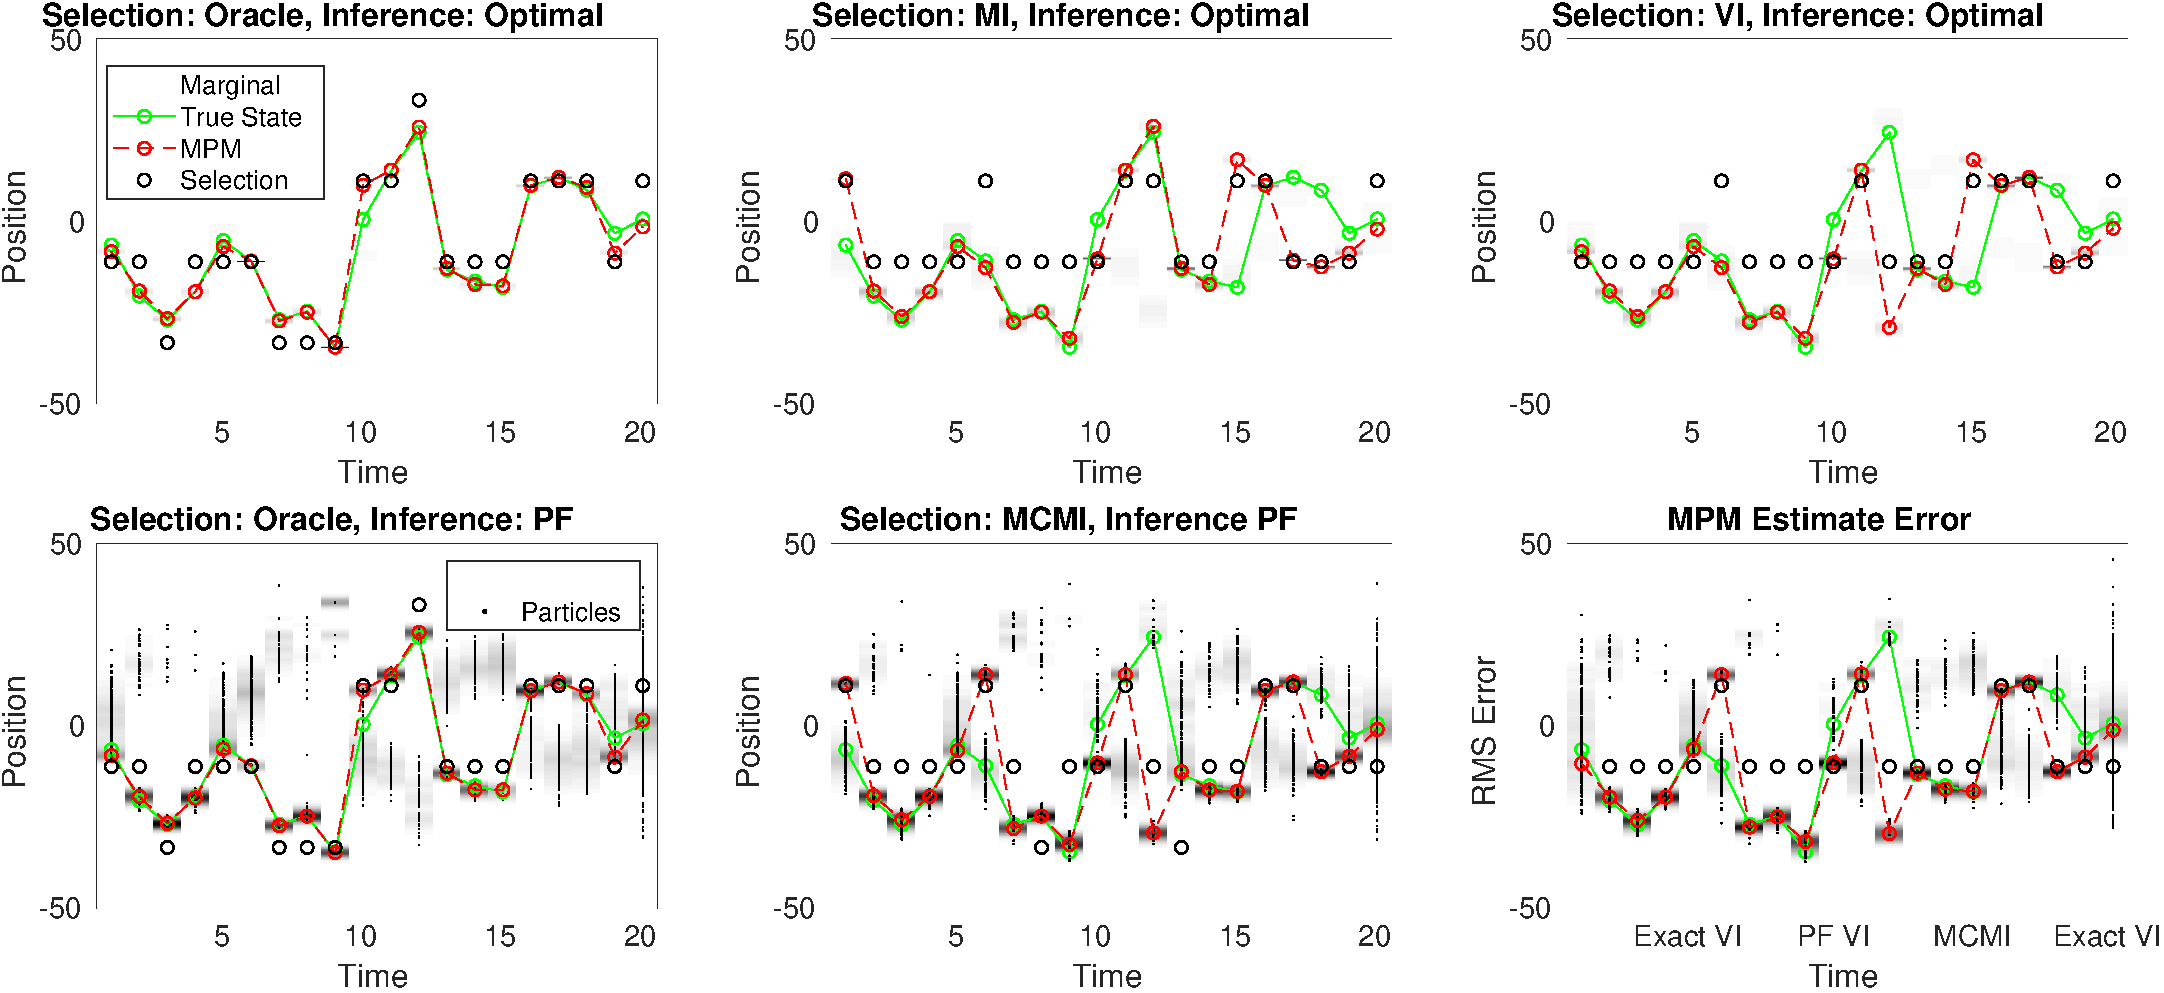
\includegraphics[width=0.9\textwidth]{tracking_single}
  \vspace{-3mm}
  \caption{\small\textbf{Nonlinear tracking example} in a field of
    $K=10$ equally spaced, stationary, sensors.  The best comparison
    is to numerical approximation to MI and the posterior distribution
    (\emph{top-center}).  For reference, we have also included an
    \emph{oracle} which selects the sensor closest to the true target
    location (\emph{left column}).  In typical cases such as this one,
    we see that VIP state error is comparable to empirical estimation
    under the same posterior approximation.  However, VIP shows lower
    accuracy when planning is computed against an approximate
    posterior, in this case particle filtering (PF).}
  \vspace{-3mm}
  \label{fig:tracking_single}
\end{figure*}

\textbf{Dynamical System.} We extend the setting above to a dynamical
system with nonlinear dynamics $p(x_t\mid x_{t-1})$ frequently used in
the sequential Monte Carlo literature~\citep{kitagawa1996monte,
  gordon1993novel, cappe2007overview},
\[
  \Ncal\left(0.5 x_{t-1} + 25 x_{t-1} / (1+x_{t-1}^2)
  + 8 \cos(1.2t), \sigma_u^2\right).
\]
To keep consistent with prior work we model observations
as, \mbox{$y_t \mid x_t; k \sim \Ncal(x_t^2/20, v_{tk}(x_t))$}.  The
variance function $v_{tk}(x_t)$ is identical to our static example.
To demonstrate flexibility additionally replace variational inference
with a particle filter.  \FIG\ref{fig:tracking_single} demonstrates an
example scenario.

\subsubsection{Results}
In both models, static and dynamic, we optimize the MI lower bound
over a linear Gaussian approximation $\omega(x \mid y_t)$, which can
be solved in closed-form.  We compare the impact of inference on
predictive accuracy by comparing exact numerical calculation,
variational inference, and MCMC.

\textbf{State predictions competitive with empirical.}  In both cases
VIP produces state estimates with similar or better accuracy to
empirical planning, depending on the chosen posterior approximation.
In the static estimation model we find similar accuracy between exact
numerical inference with empirical planning and EP inference with VIP
planning (\FIG\ref{fig:static}; left).  In the tracking model we also
consider exact inference with VIP planning, for which median error is
lowest.  When comparing particle filter inference VIP and empirical
planning accuracy are comparable, with the former showing slightly
lower median error (\FIG\ref{fig:dynamic}; left).

\textbf{Planning is sensitive to posterior accuracy.}  We also find
that estimates of the state estimate, and of the MI calculation, are
sensitive to accuracy of the posterior approximation.  In the static
case we compare against assumed density filtering (ADF), which is more
numerically stable than EP but tends to produce less accurate
posterior approximations.  Planning based on the ADF posterior
produces less accurate state estimates (\FIG\ref{fig:static}; left)
and higher error MI estimates (\FIG\ref{fig:static}; right).
Similarly, use of particle filter inference in the tracking model
increases error for both the state (\FIG\ref{fig:dynamic}; left) and
MI calculation (\FIG\ref{fig:dynamic}; right).



\begin{figure}[t]
  \begin{tabular}{cc}
    \hspace{-3mm}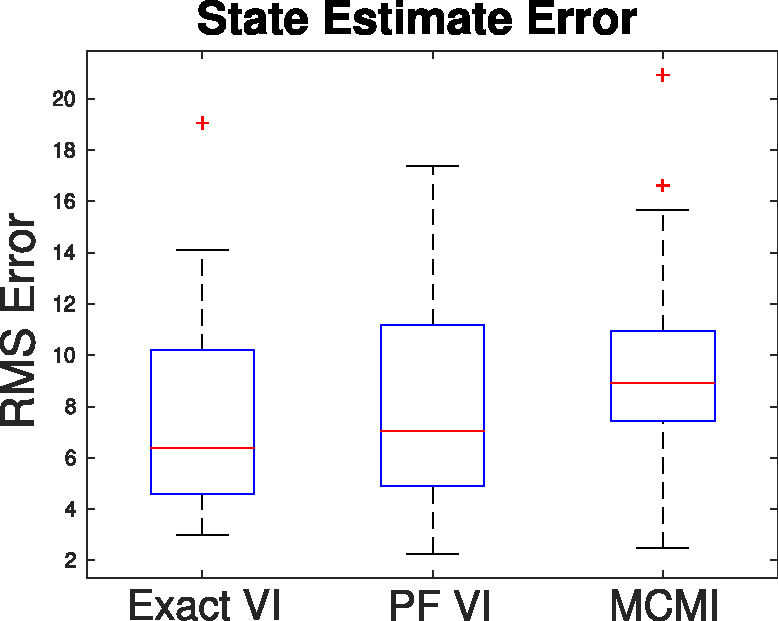
\includegraphics[width=0.23\textwidth]{tracking_state_err} &
    \hspace{-3mm}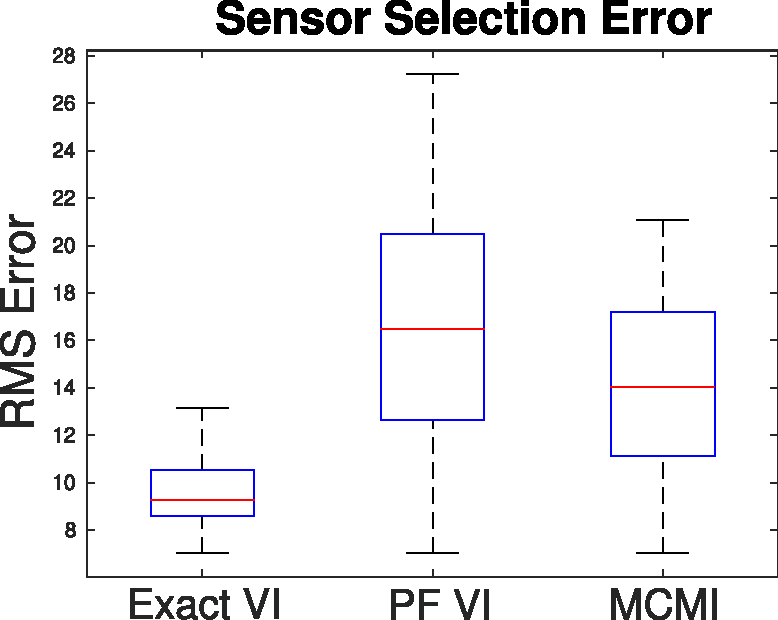
\includegraphics[width=0.23\textwidth]{tracking_sensor_err}
  \end{tabular}
  
  \caption{\small\textbf{Nonlinear tracking for 20 random
  trials.}  \emph{Left:} Exact inference with variational planning
  yields the lowest RMS state error.  Particle filter inference with
  500 particles and variational planning (PFVI) yields lower median
  error compared to MC estimates of information (MCMI), though wider
  error quantiles.  \emph{Right:} Again, Exact VI shows the lowest RMS
  error of the selected sensor position w.r.t.~optimal, whereas PFVI
  and MCMI both have higher error, again with PFVI having larger
  quantiles.}\vspace{-5mm}
  \label{fig:dynamic}

\end{figure}





\subsection{Gene Regulatory Network}

Next, we demonstrate VIP for Bayesian experimental design in the
discovery of causal gene interactions.  Specifically, we develop our
approach for the sparse linear model of \cite{steinke2007experimental,
  seeger2008bayesian}.

Let $x\in\RR^n$ represent the deviation of $n$ gene expression levels
from steady state.  The matrix $A\in\RR^{n\times n}$ represents causal
interactions, with sparse entries drawn independently from a Laplace
distribution.  The model is,
\begin{equation}\label{eq:sparselin}
  \!\!\!p(A,x) \propto \prod_{i=1}^n \Ncal(u_i \mid a_i^T
    x, \sigma^2) \prod_{j=1}^n \textrm{Laplace}(a_{ij} \mid \lambda) 
\end{equation}
where $a_i$ is the $i^{\text{th}}$ row of matrix $A$.  Here $u$
represents an external control vector (perturbation).  Interventions
include up regulating $u_i>0$, down regulation $u_i<0$ and no
intervention $u_i=0$ for the $i^{\text{th}}$ gene.  Observe that the
joint~\eqref{eq:sparselin} is defined up to normalization since the
likelihood term is not a normalized distribution of $x$.

\begin{figure}[t]
  \centering
  \begin{tabular}{cc}
    \hspace{-3mm}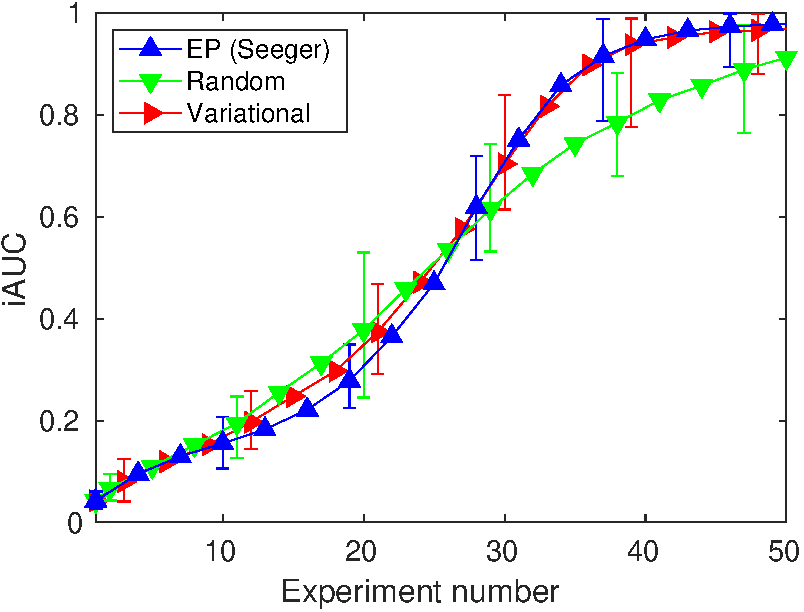
\includegraphics[width=0.24\textwidth]{sparselin_iAUC_N100_norandom_run20_norepeats} &
    \hspace{-3mm}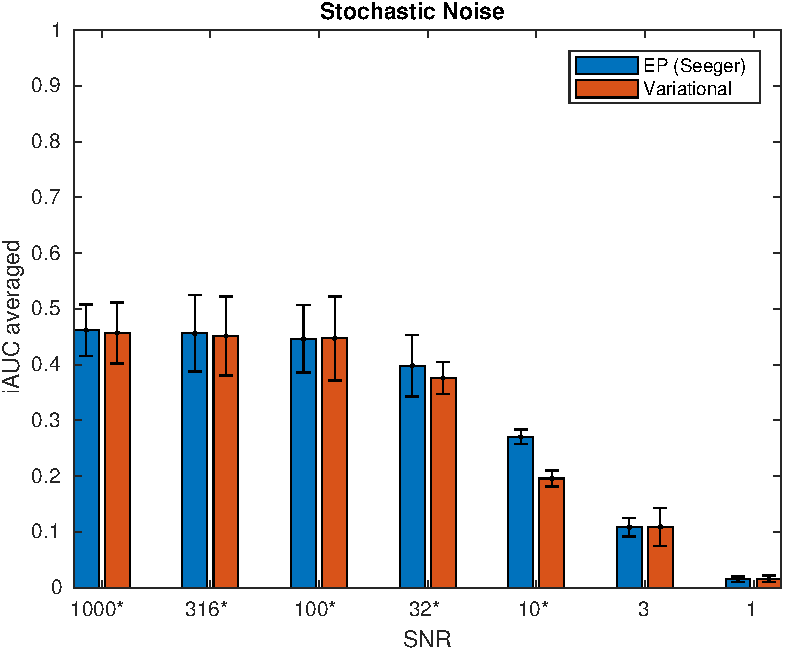
\includegraphics[width=0.22\textwidth]{sparselin_noise_N100_norandom_run20_norepeats}
  \end{tabular}
  \caption{\small\textbf{Sparse linear model.} Average +/- STDEV
    computed for $n=50$ nodes over 20 random networks.  \emph{Left:}
    AUC for edges with true weights $|a_{ij}|>0.1$ plotted for each
    intervention experiment.  VIP shows similar results to Steinke and
    Seeger with slight improvement for less than 25 experiments.
    \emph{Right:} Average AUC at varying noise levels are broadly
    similar to Steinke and Seeger. The dip at moderate SNR levels may
    be due to our choice of a simple approximating family (linear
    Gaussian).}
  
  \label{fig:sparselin}
\end{figure}

As exact inference is infeasible, we instead compare to the method
developed in \cite{steinke2007experimental, seeger2008bayesian}, which
maintains a mean field Gaussian posterior approximation using EP,
\mbox{$q(A) = \prod_i p_i^{(0)}(a_i) \prod_j
  \widetilde{t}_{ij}(a_{ij})$}.  Here, $p^{(0)}_i(a_i)$ approximates
the base measure \mbox{$N(u_i \mid a_i^T x, \sigma^2)$} and
\mbox{$\widetilde{t}_{ij}(a_{ij})$} the Laplace factors.

Given past observations $\Dcal$ and a new control and observation pair
$\{x_*,u_*\}$, maximizing MI is (approximately) equivalent to
maximizing \mbox{$\EE_{x_*}\!\left[\, \KL{q'}{q} \,\right]$},
%% \begin{equation}\label{eq:max_kl}
%%   \max_{u_*} \; \EE_{x_*}\!\left[\, \KL{q'}{q} \,\right],
%% \end{equation}
where approximation comes from the update posterior \mbox{$q'(A)
  \approx p(A \mid \Dcal \cup \{x_*,u_*\})$}.  The previous authors
approximate expectation over samples $\{x_{*}^{k}\}$ from the
predictive distribution $p(x_{*} \mid \Dcal, u_{*})$.  Since this
approach requires updating the EP posterior $q'(A)$ for each sample
$x_{*}^k$, which is prohibitive, they instead propose a
non-iterative approximation which only updates the Gaussian base measure
$p^{(0)}(A)$ at each sample.

\textbf{Similar results to specialized method.} We optimize the MI
bound over a linear Gaussian approximation for 20 random trials and
report area under the curve (AUC) for edge prediction
(\FIG\ref{fig:sparselin}; left).  Steinke and Seeger approximate MI by
updating only the base measure $p^{(0)}$, which involves a moment
matching projection $\EE_{q'}[ \phi(A) ] = \EE_{\hat{p}}[ \phi(A) ]$,
where $\hat{p}(A)$ is the augmented distribution, which is similar to
the moment matching solution discussed in \SEC\ref{sec:moment_match}.
As a result, VIP reduces to a solution similar to that of Steinke and
Seeger, and results are comparable for more than 30 interventions.
Results remain similar across varying noise levels
(\FIG\ref{fig:sparselin}; right), albeit with a slight drop in
accuracy at moderate SNR.  We hypothesize that this intermediate
region depends more strongly on good MI approximations, and that VIP
would benefit from a more flexible approximating distribution than the
linear Gaussian one chosen.


\textbf{Improved AUC for fewer interventions.}  Despite similarity in
the methods, we do observe small improvements at early interventions.
In particular, Steinke and Seeger observe that their proposed
experimental design approach performs poorly for few interventions and
propose a hybrid method which randomly selects the first 20
interventions, then performs information guided selection thereafter.
Random selection still performs well in this regime.

%% which matches
%% moments of $q^{'}$ to those of.  Specifically, the
%% augmented distribution is given by,
%% \[
%%   \hat{p}(a_i, x_*) \propto \Ncal(u_* \mid a_i^T
%%   x_*, \sigma^2) \prod_j \widetilde{t}_{ij}(a_{ij}).
%% \]
%% The EP update then matches moments to the augmented distribution above
%% for each row $a_i$.
%% %% $\EE_{\hat{p}}[a_i] = \EE_{q'}[ a_i ]$ and $\text{var}_{\hat{p}}[ a_i
%% %% ] = \text{var}_{q'}[ a_i ]$ for each row $a_i$.
%% %% \[
%% %%   q' \Leftrightarrow \argmin_{q'} \KL{}{q'}
%% %% \]

\subsection{Active Learning for Labeled LDA}\label{sec:llda}

%% \begin{figure*}
%%   \begin{tabular}{cccc}
%%     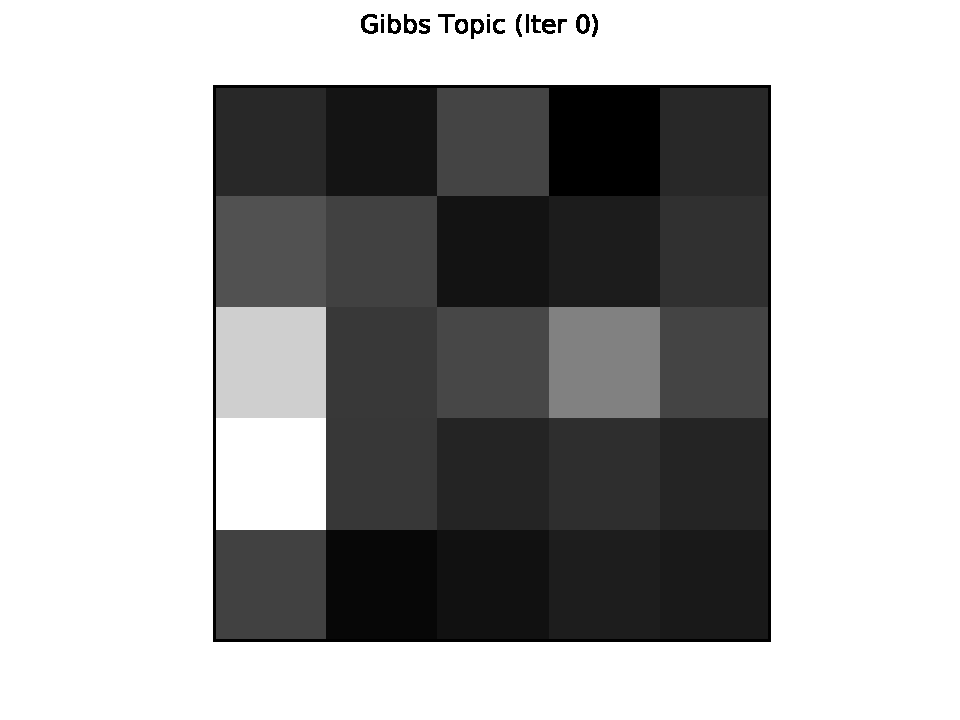
\includegraphics[width=0.24\textwidth]{llda/Gibbs_iter0} &
%%     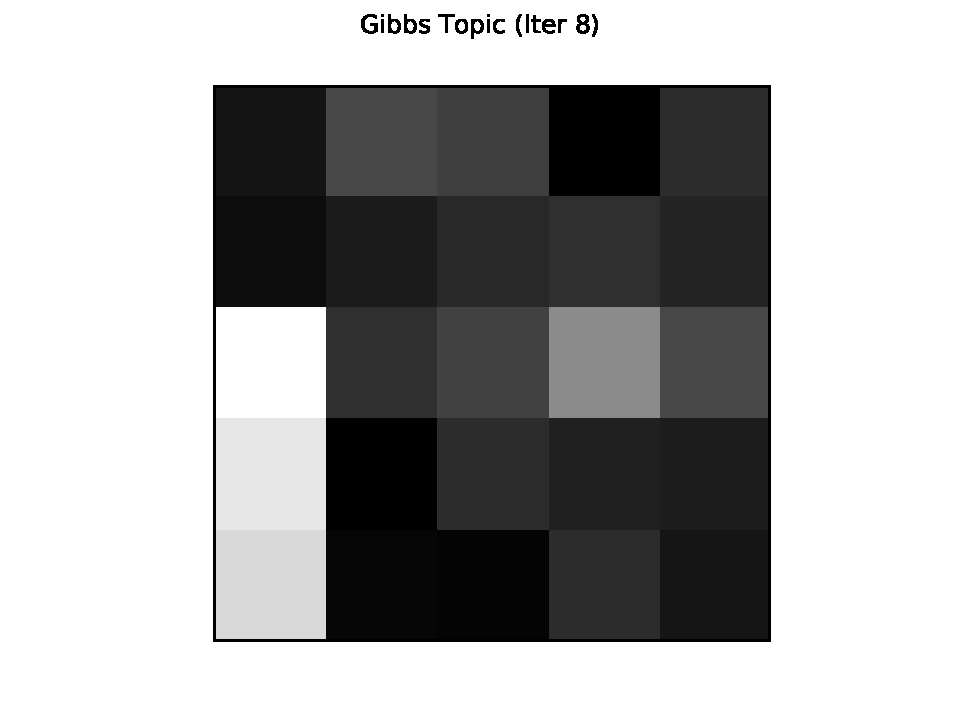
\includegraphics[width=0.24\textwidth]{llda/Gibbs_iter8} &
%%     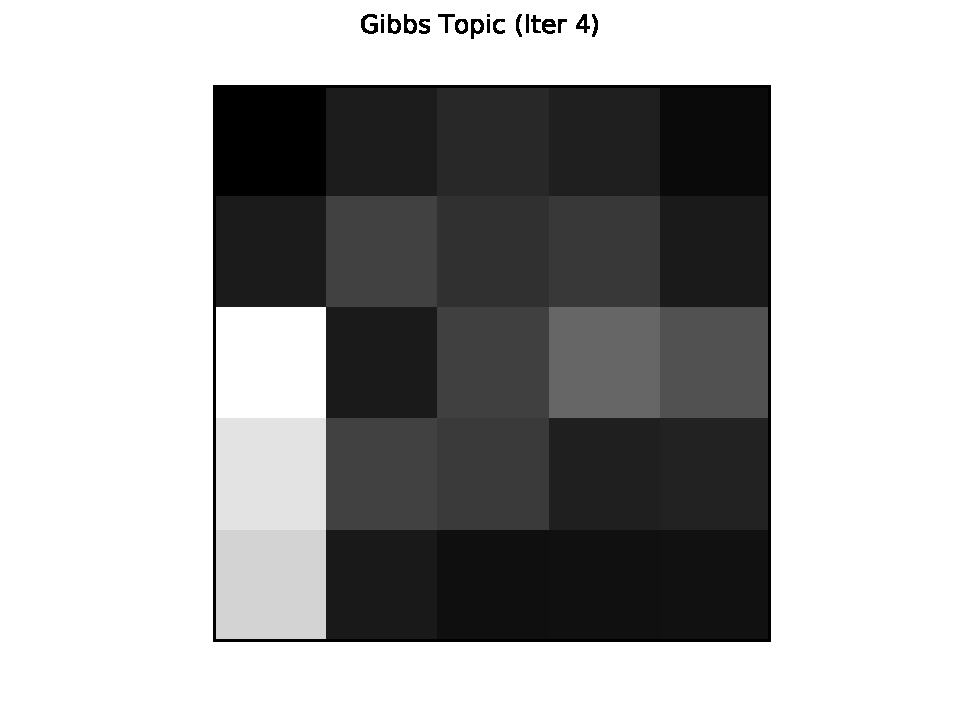
\includegraphics[width=0.24\textwidth]{llda/Gibbs_iter4} &
%%     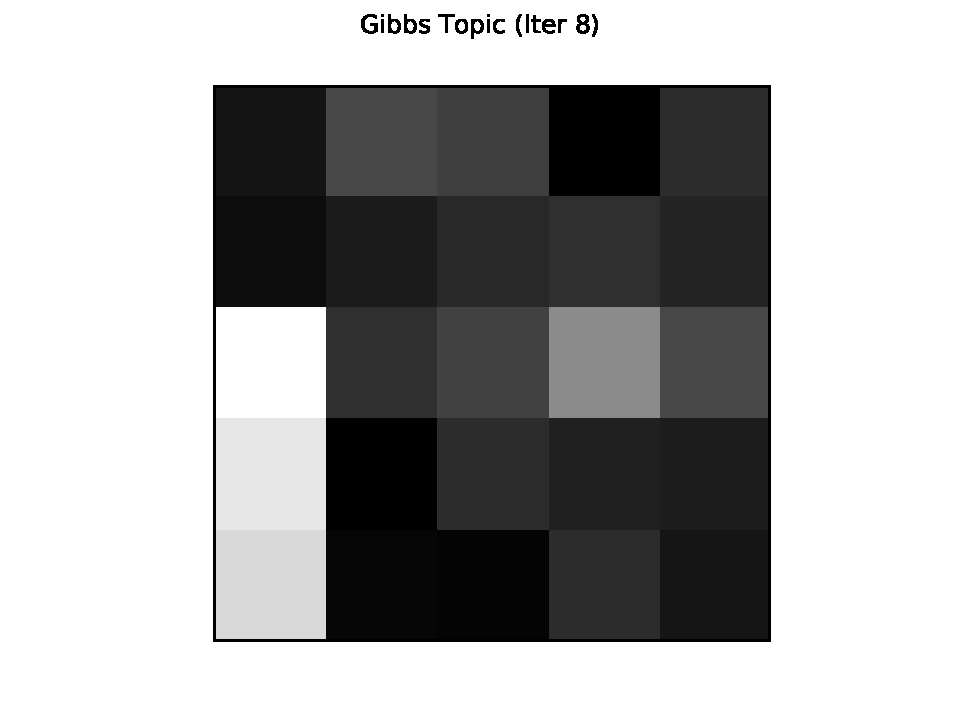
\includegraphics[width=0.24\textwidth]{llda/Gibbs_iter8} \\
    
%%     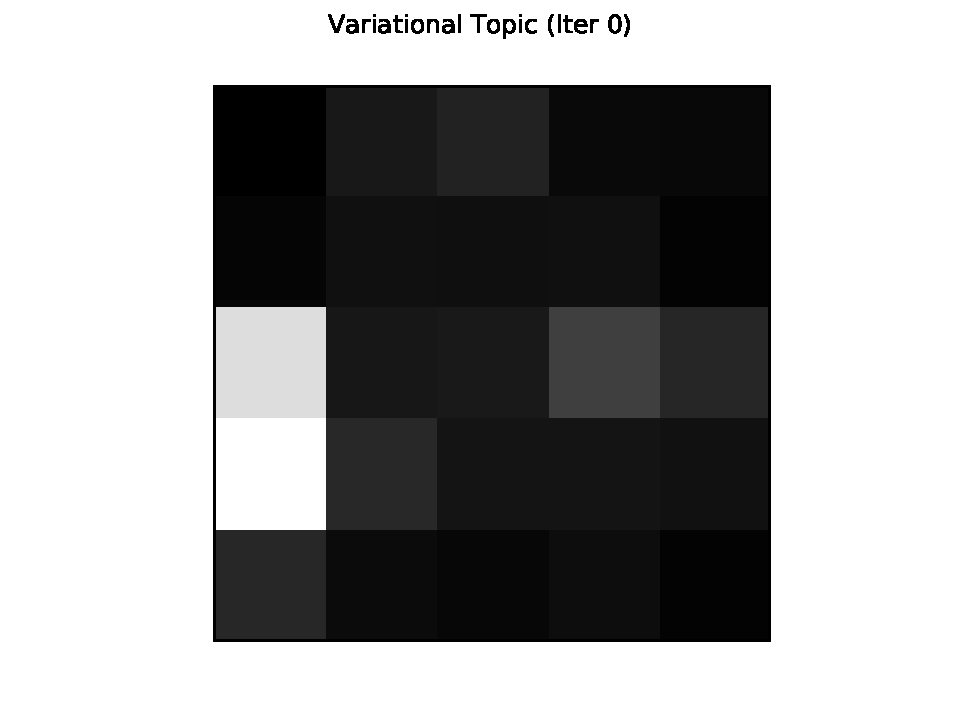
\includegraphics[width=0.24\textwidth]{llda/Variational_iter0} &
%%     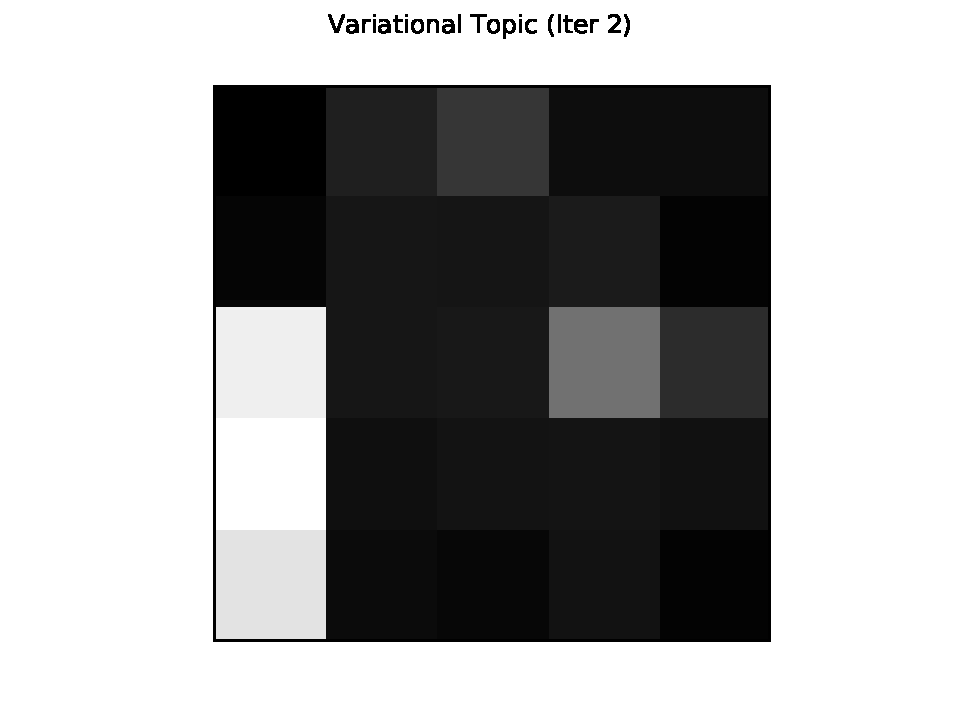
\includegraphics[width=0.24\textwidth]{llda/Variational_iter2} &
%%     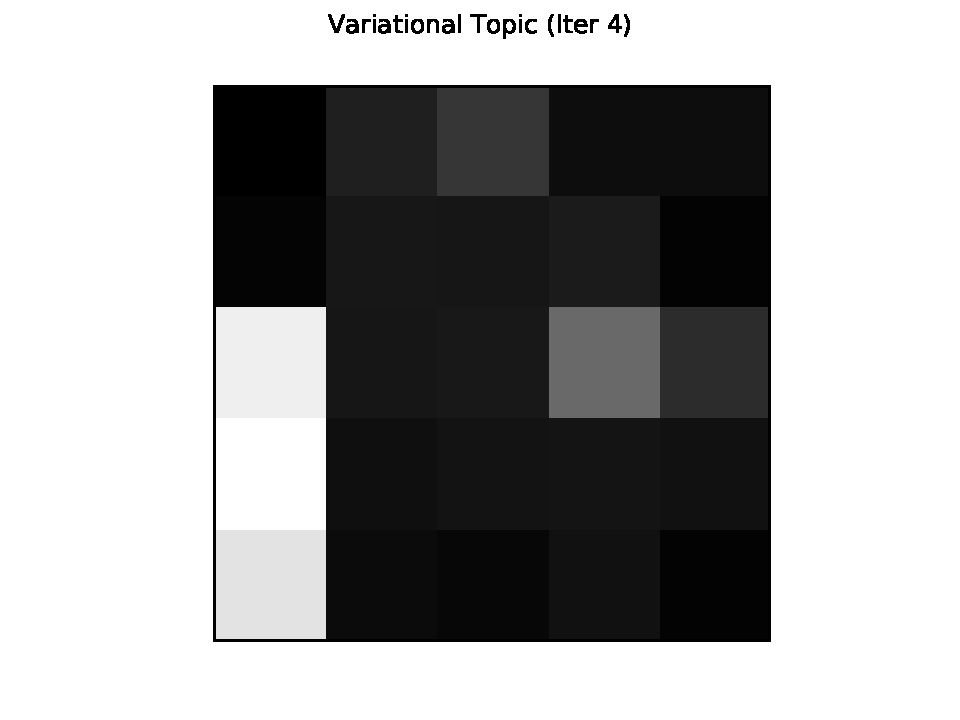
\includegraphics[width=0.24\textwidth]{llda/Variational_iter4} &
%%     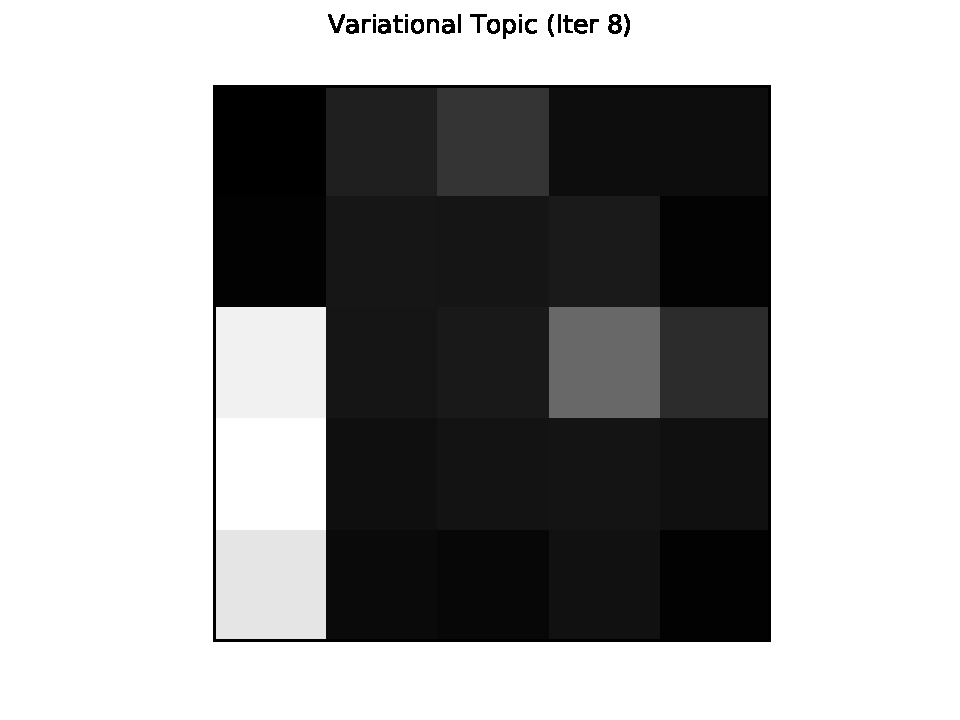
\includegraphics[width=0.24\textwidth]{llda/Variational_iter8}
%%   \end{tabular}
%%   \caption{\small\textbf{Labeled LDA.} Blah.}
%% \end{figure*}

\begin{figure*}
  \begin{tabular}{ccc}
    \hspace{-3mm}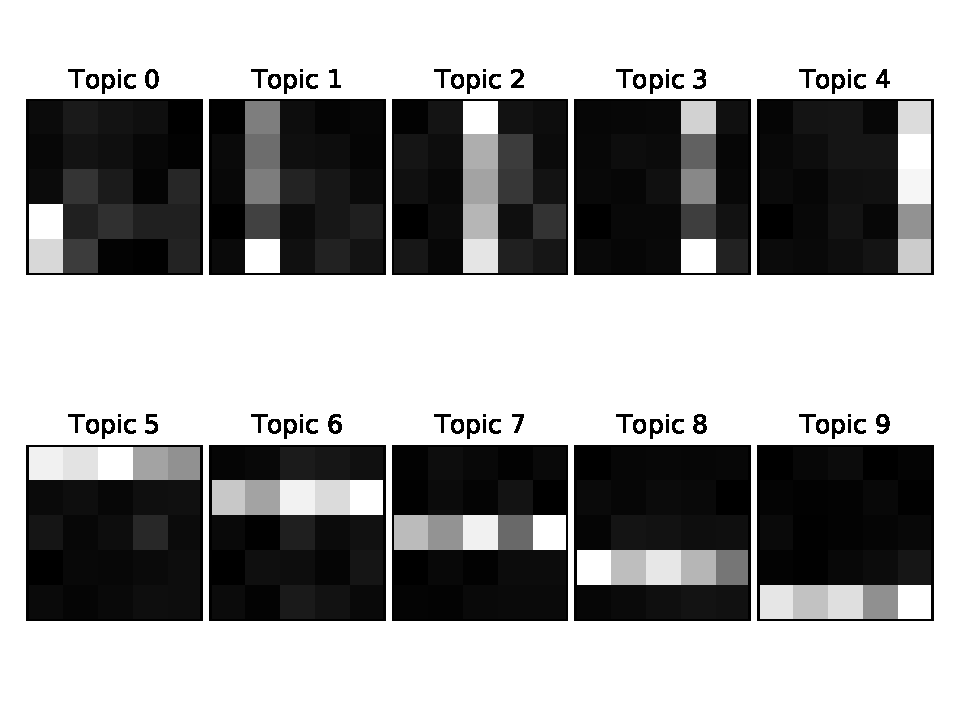
\includegraphics[width=0.32\textwidth]{llda/topics_random_runid_5} &
    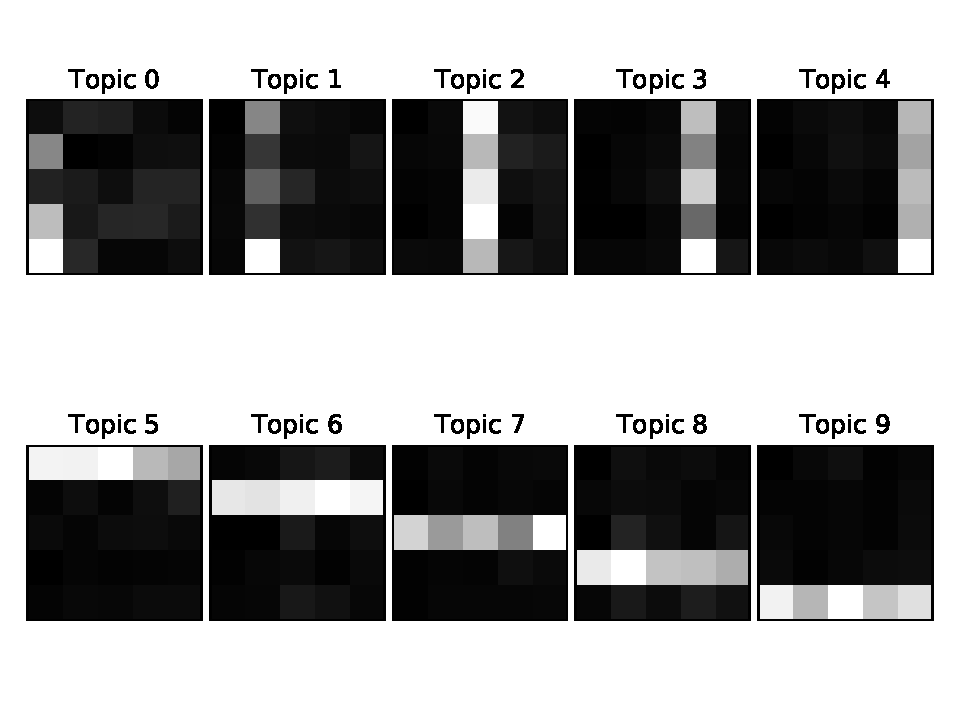
\includegraphics[width=0.32\textwidth]{llda/topics_gibbs_runid_5} &
    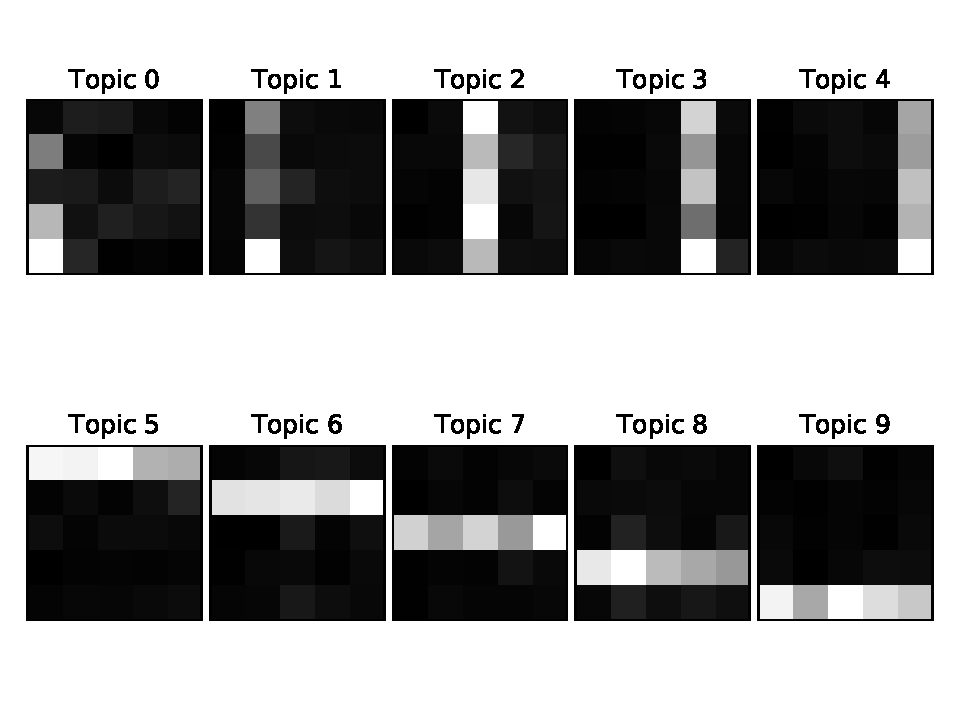
\includegraphics[width=0.32\textwidth]{llda/topics_vip_runid_5} \vspace{-3mm}\\
    {\small\textbf{Gibbs + Random}} & {\small\textbf{Gibbs +
        Empirical}} & {\small\textbf{EP + VIP}}
  \end{tabular}

  \caption{\small \textbf{Learned LLDA topics} from a corpus of $D=50$
    documents, each with $N_d=25$ words drawn from the bars topics
    with a $W=25$ word vocabulary.  We model Topic 0 as a \emph{rare}
    topic (see text).  Gibbs estimates are averaged over $1000$
    samples drawn from parallel chains.  Topic estimates under EP
    inference with selection using VIP (\emph{right}) are broadly
    similar to Gibbs when using empirical MI estimates for selection
    (\emph{center}), though at reduced computational cost.  Gibbs
    estimates have higher noise in low probability regions.
    Annotation based on random selection (\emph{left}) performs poorly
    regardless of the inference method -- Gibbs shown.}
  \vspace{-5mm}
  \label{fig:llda_topics}
\end{figure*}

\begin{figure}[t]
  \centering
  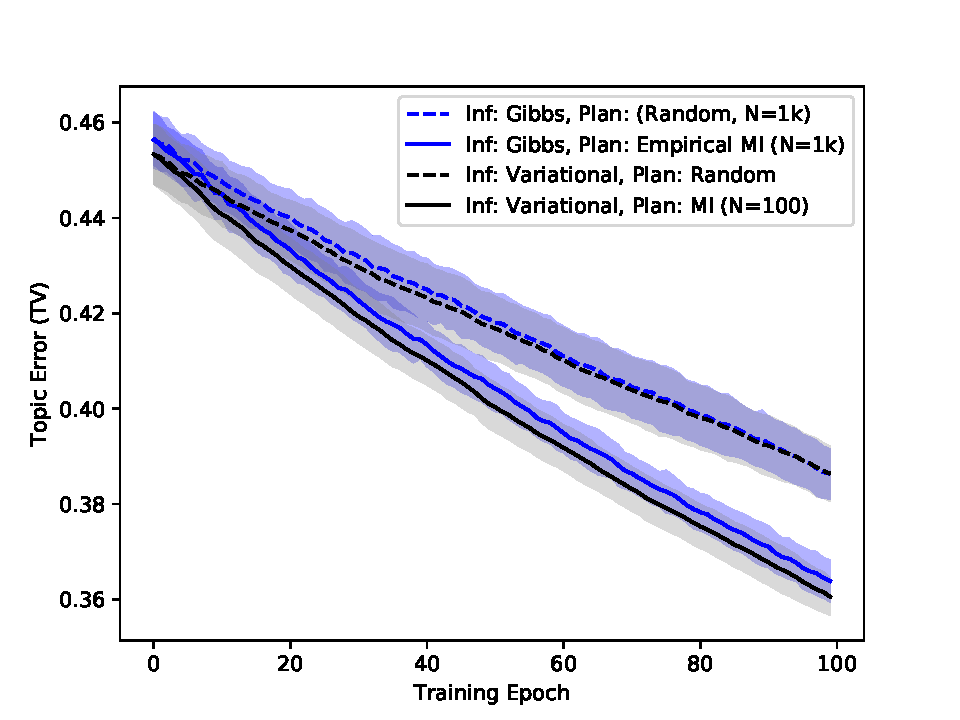
\includegraphics[width=0.45\textwidth]{llda/llda_tverr} \vspace{-2mm}
  
  \caption{\small\textbf{Labeled LDA.} Total variation error (absolute
  error) for all topics on the ``bars'' dataset across 10 random
  trials.  Variational planning with fully parameterized softmax shows
  consistent improvement over Gibbs on average (solid).  Gibbs
  estimates show tighter standard deviation (shaded) for planning
  based on MI estimates.  Both inference methods perform similarly
  for random selection.}
  
  \label{fig:llda_tv}
\end{figure}

\begin{figure}[t]
  \centering
  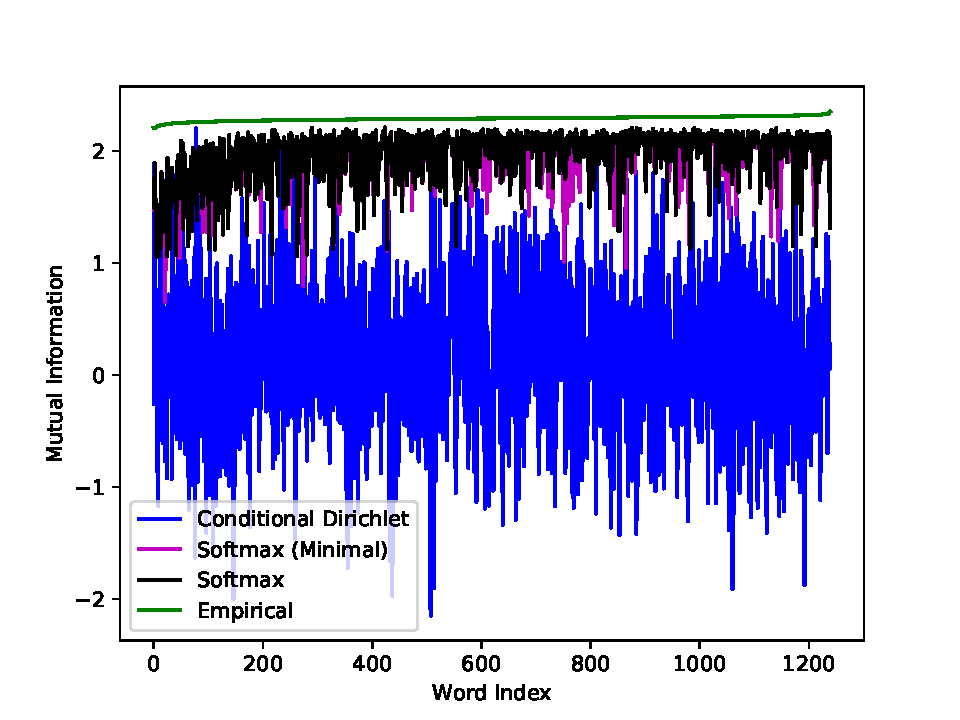
\includegraphics[width=0.45\textwidth]{llda/bound_comparison}
  
  \caption{\small\textbf{LLDA Bound Comparison.} Variational MI
  estimates for annotations using three approximating families, ranked
  in order of increasing value by empirical estimate of MI.  An ideal
  approximation would show monotonically increasing values with little
  gap.  The conditional Dirichlet model is a poor approximation.  Two
  variations on the softmax distribution provide tighter bounds, with
  the fully parameterized softmax being slightly
  preferred.}  \label{fig:llda_bound}
\end{figure}

Labeled LDA (LLDA) is one of several proposed semi-supervised
extensions to LDA~\citep{blei2003latent}.  The standard unsupervised
LDA model is given by,
\begin{align*}
  \theta_d &\sim \text{Dirichlet}(\alpha), &&\text{For}\; d=1,\ldots,D \\
  \psi_k &\sim \text{Dirichlet}(\beta_k), &&\text{For}\; k=1,\ldots,K \\
  z_{dn} \mid \theta_d &\sim \text{Cat}(\theta_d), &&\text{For}\;
    n=1,\ldots,N_d \\
  w_{dn} \mid z_{dn}, \psi &\sim \text{Cat}(\psi_{z_{dn}}) &&
\end{align*}
LLDA augments the standard LDA model with semi-supervised annotations
for each word~\citep{flaherty2005latent}.  We model annotations as
noisy observations of the true topic assignment: \mbox{$y_{dn} \mid
  z_{dn} \sim \text{Cat}(\pi_{z_{dn}})$}.  In this way, annotations
induce a preferred ordering of topic labels in the posterior,
producing interpretable topics.  There are variations on this
approach~\citep{ramage2009labeled} which model annotations at the
document level, but we do not consider them here.

We perform active learning, which falls under the annotation model of
\SEC\ref{sec:annotation}.  At each learning stage $t$, the planner
selects an annotation $y_{d^*n^*}$ maximizing MI over the topics,
\begin{equation}
  (d^*,n^*) = \argmax_{(d,n)} I(\Psi, Y_{dn} \mid \Wcal, \Ycal_{t-1}),
\end{equation}
given the observed corpus of words $\Wcal$ and previous annotations
$\Ycal_{t-1}$.  We demonstrate active learning on the ``bars''
data~\citep{griffiths2004finding} in which topics can be arranged and
visualized as a set of vertical and horizontal \emph{bars} (see
\FIG\ref{fig:llda_topics}).  To amplify the effect of poorly informed
selections we additionally model a \emph{rare} topic by setting a
non-symmetric Dirichlet prior on topic proportions: $\alpha = (0.05,
1, 1, \ldots, 1)^T$.

Empirical MI estimates based on Gibbs samples involve averages across
independent MCMC chains, and are thus sensitive to topic label
switching~\citep{stephens2000dealing}.  We found that alignment to any
individual sample (e.g. MAP) produced poor results, both in terms of
the posterior mean estimate of the topics as well as entropy
estimates.  We instead relabel Gibbs samples to minimize absolute
error w.r.t.~the ground truth topics.  Such an approach would not be
feasible in typical cases as it requires knowledge of the true topics,
but represents the best achievable estimate over the given samples.  Our
variational planning approach does not suffer similar issues as
samples are drawn from a consistent topic posterior distribution.

\textbf{Lower topic error compared to Monte Carlo.}
\FIG\ref{fig:llda_tv} reports total variation (TV) error across topics
$\sum_k \|\psi_k - \hat{\psi}_k\|_1$, based on the posterior mean
estimate $\hat{\psi}$.  The TV error is invariant to topic ordering
as we solve a bipartite matching to compute the lowest TV error across
labels.  Increasing MCMC samples from the reported 1000 samples does
not lead to significant improvements.  We instead suspect that poor
MCMC results are due to a combination of MI estimator bias, inference
local optima, and topic label switching.

\textbf{More flexible approximations lead to better bounds.}  We
consider three forms of the auxiliary distribution $\omega(\cdot)$ in
the MI lower bound: a conditional Dirichlet, $\omega(\psi \mid y=j) =
\prod_k \text{Dirichlet}(\psi_k \mid \gamma_{kj})$, a \emph{minimal}
softmax where class conditionals depend on a single topic $\omega(y =
k \mid \psi) \propto \exp( w_k^T \text{vec}(\psi_k) + w_{0k} )$, and
where class conditionals weight all topics \mbox{$\omega(y = k \mid
  \psi) \propto \exp( w_k^T \text{vec}(\psi) + w_{0k}
  )$}. \FIG\ref{fig:llda_bound} compares variational MI estimates to
that of an empirical estimate for each of these families.  We find
that the larger parameter set of this final family leads to more
accurate bounds overall.


%% MI as $I(\Psi,Y_{dn}) \geq H(Y_{dn})
%% + \EE[ \log \omega(Y_{dn} \mid \Psi) ]$ using the following softmax
%% distribution,
%% \begin{equation}
%%   \omega(Y = k \mid \Psi) \propto \exp( w_k^T \text{vec}(\Psi) +
%%   w_{0k} ).
%% \end{equation}

%% which is in the exponential family with natural parameters
%% $\theta(\Psi) = (w_1^T \text{vec}(\Psi) + w_{01}, \ldots,
%% w_K^T \text{vec} + w_{0K})^T$.





